\documentclass[floatfix,aps,pra,twocolumn,superscriptaddress,10pt,nofootinbib]{revtex4-2}
% Starter manuscript for the inverse problem. On the first Overleaf sync it is replaced by the
% Overleaf project if that project already holds a draft (see README, "Paper and Overleaf").

\usepackage{graphicx}
\usepackage{bm}
\usepackage{booktabs}
\usepackage{amsmath,amssymb}
\usepackage{xcolor}
\usepackage{hyperref}

% Same colours as the forward-problem paper: quantum = orange, classical = blue
\definecolor{qcol}{HTML}{EB6834}
\definecolor{ccol}{HTML}{2A78D6}

\newif\ifshowtodos \showtodostrue
\newcommand{\TODO}[1]{\ifshowtodos\textcolor{red}{\textbf{[TODO:} #1\textbf{]}}\fi}
\newcommand{\Ncol}{N_{\rm col}}

\hypersetup{colorlinks=true, linkcolor=blue!50!black, citecolor=blue!50!black, urlcolor=blue!50!black}
\graphicspath{{figures/}}

\begin{document}

\title{Inferring the viscosity of Burgers' equation with a hybrid quantum physics-informed neural network}

\author{Gubio G. de Lima}
\email{gubio.gomes@estudante.ufscar.br}
\affiliation{\TODO{afilia\c{c}\~ao (CBPF / UFSCar)}}

\begin{abstract}
\TODO{Resumo -- a escrever por \'ultimo.}
\end{abstract}

\maketitle

\section{Introduction}\label{sec:intro}
\TODO{Inverse problems with PINNs; why a fixed quantum layer; what is new here.}

\section{Inverse problem}\label{sec:problem}
We consider the viscous Burgers equation
\begin{equation}
  u_t + u\,u_x = \nu\,u_{xx}, \qquad x \in [0, 1) \text{ periodic}, \quad u(x, 0) = \sin(2\pi x),
\end{equation}
with the viscosity $\nu$ unknown. The true value is $\nu = 0.01$, and we study two final times,
$T = 0.1$ and $T = 1$; for $T = 1$ a shock forms before the final time. At every epoch, $\Ncol = 10$
new collocation points $(x_c, t_c)$ are drawn at random in $[0, 1) \times [0, T]$. They are used twice:
for the residual of the equation and as data, the exact (Cole--Hopf) solution at the same points.
The network is trained on both, and $\nu$ is learned together with it~\cite{raissi2019physics}.

\section{Models and training}\label{sec:methods}
Both models share the same structure: a pre-network maps $(\sin 2\pi x, \cos 2\pi x, t/T)$ to $k$
features, a middle block transforms them, and a post-network maps them to $u$ (one hidden layer of 10
$\tanh$ units in each network). In the classical PINN the middle block is a trainable bottleneck of
$k = 3$, 7 or 10 neurons. In the hybrid quantum PINN it is a fixed circuit on $k = 3$, 7 or 10 qubits:
the features enter as $R_Y$ angles, followed by a brickwork layer of CNOTs, and the outputs are the
expectation values $\langle Z_i\rangle$. The circuit is evaluated on the FakeBerlin emulator of the
\texttt{ibm\_berlin} device (1024 shots) with the device in the training loop: one job per epoch, with
the gradient taken through a polynomial calibrated on the device.

The residual $u_t + u u_x - \nu u_{xx}$ is computed by finite differences on a 5-point stencil around
each collocation point, and split as $A - \nu B$. The network is trained with AdamW on the loss
$\lambda_r\,\mathrm{MAE}(A - \nu B) + w_d\,\mathrm{MAE}(u - u_{\rm data})$, with 16 steps per epoch,
$w_d \gg 1$ and $\lambda_r$ ramping from 0 to 1 in the first epochs. With the network fixed, the $\nu$
that minimizes the residual of the batch is the $|B|$-weighted median of $A/B$, and $\log\nu$ is
relaxed towards it at every epoch. Training stops after 110 epochs.

For $T = 1$ three changes are needed to represent the shock: the initial condition enters as a loss
on 10 random points at $t = 0$ instead of being imposed exactly, the first 10 epochs use the data loss
only with $\nu$ frozen, and the learning rate is cut on plateaus of the loss instead of decaying as a
cosine. Both models use the same changes.

\section{Results}\label{sec:results}

\begin{figure*}
  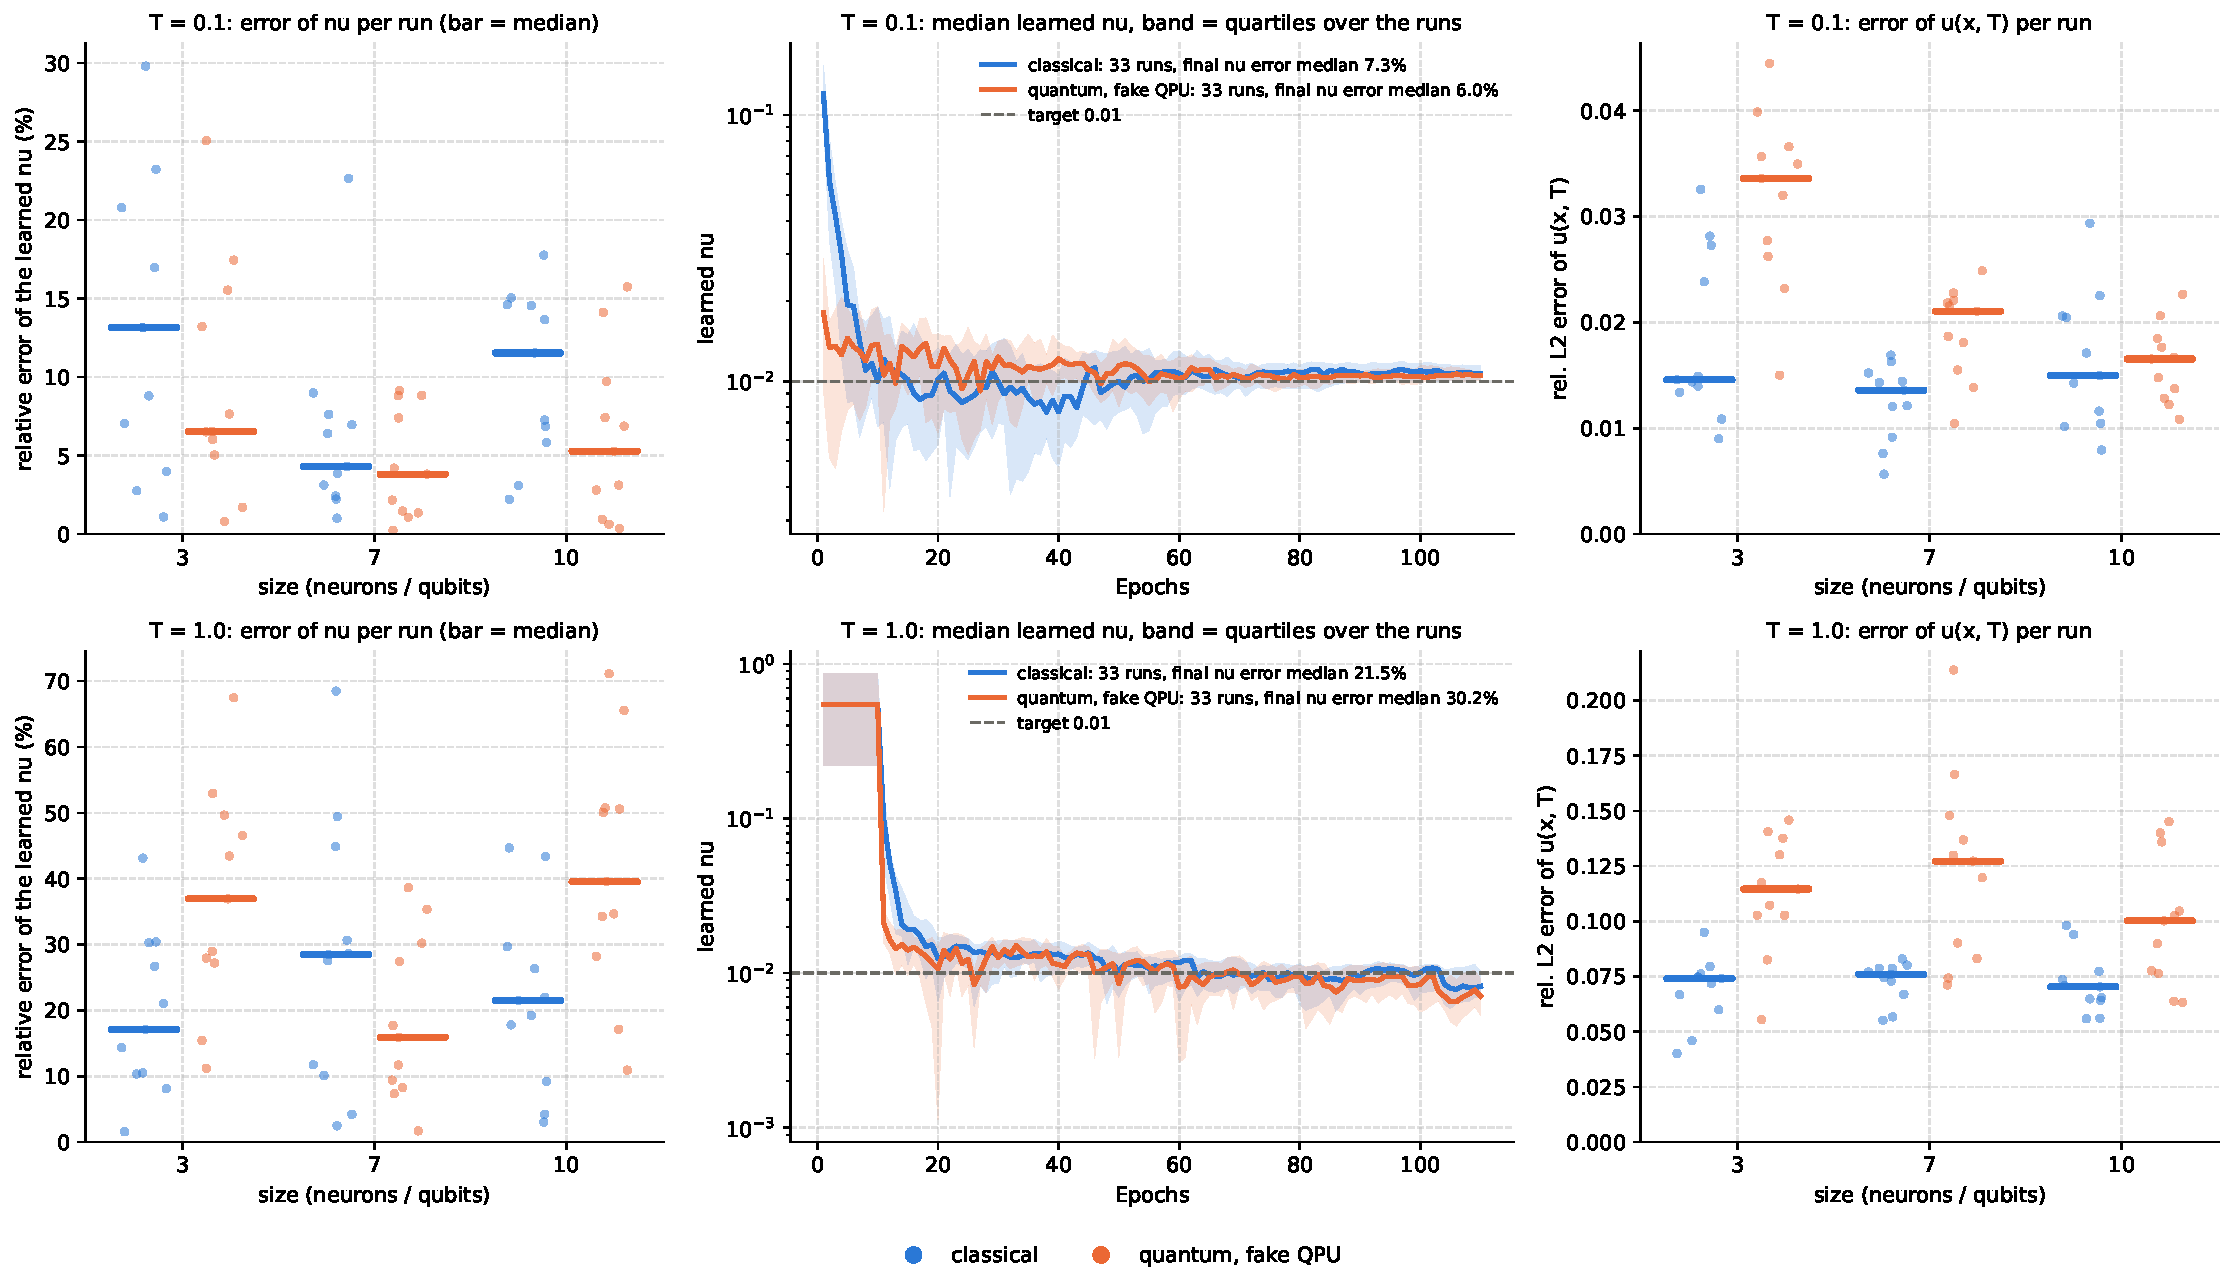
\includegraphics[width=\textwidth]{comparacao_classico_quantico_nu_0.01_E110.pdf}
  \caption{Classical (blue) and hybrid quantum PINN on the FakeBerlin emulator (orange), $\nu = 0.01$,
  110 epochs, $\Ncol = 10$, for $T = 0.1$ (top) and $T = 1$ (bottom). Left: relative error of the
  learned $\nu$ in each of the 33 runs per model (3, 7 and 10 neurons or qubits $\times$ 11 seeds); the
  bars are the medians. Middle: median of the learned $\nu$ over the runs, against the epoch, with the
  interquartile band. Right: relative $L_2$ error of $u(x, T)$ in each run. Generated by
  \texttt{run/plots/plot\_inverse\_E110.py}.}
  \label{fig:comparison}
\end{figure*}

\begin{table}
  \caption{Relative error of the learned $\nu$ (median and 90th percentile) and median relative $L_2$
  error of $u(x, T)$ over 33 runs per model ($\nu = 0.01$, 110 epochs).}
  \label{tab:results}
  \begin{ruledtabular}
  \begin{tabular}{llccc}
    $T$ & model & $\nu$, median & $\nu$, p90 & $L_2$ of $u$ \\
    \hline
    0.1 & classical & 7.3\% & 20\% & 0.014 \\
    0.1 & quantum   & 6.0\% & 15\% & 0.021 \\
    1   & classical & 21.5\% & 44\% & 0.073 \\
    1   & quantum   & 30.2\% & 53\% & 0.107 \\
  \end{tabular}
  \end{ruledtabular}
\end{table}

Figure~\ref{fig:comparison} and Table~\ref{tab:results} summarize the 33 runs of each model. For
$T = 0.1$ the two models estimate $\nu$ equally well: the quantum PINN has the smaller median error
(6.0\% against 7.3\%) and fewer large errors, but the difference is not significant ($p = 0.11$). The
classical PINN fits $u(x, T)$ better ($L_2$ error 0.014 against 0.021, $p < 0.001$). For $T = 1$, with
the shock, the problem is harder for both models, and the classical PINN is better in $\nu$ (21.5\%
against 30.2\%, $p = 0.046$) and in $u(x, T)$ (0.073 against 0.107). Both models underestimate $\nu$
in most of the runs at $T = 1$. With only ten points per epoch, the learned $\nu$ still moves from one
epoch to the next at the end of the training, so the error of a single run depends on the last
batches; the comparison therefore relies on many seeds.

\TODO{Dependence on the model size; effect of $\Ncol$ (more points per epoch reduce the error).}

\section{Conclusions}\label{sec:conclusions}
\TODO{Main findings: tie at $T = 0.1$, classical better at $T = 1$; outlook (more points per epoch, real device).}

\bibliography{references}

\end{document}
